\RequirePackage[svgnames]{xcolor}

\documentclass[a4paper,english,10pt,NET]{tumarticle}

% TUM packages
\usepackage{tumfonts}
\usepackage{tumarticle}
\usepackage{tumlocale}
\usepackage{tumcmd}

\usepackage{graphicx}
\usepackage[style=american]{csquotes}
\usepackage{hyperref}
\usepackage{xspace}

\usepackage{tabularx}
\usepackage{booktabs}
\usepackage{pdflscape}

\usepackage{siunitx}
\usepackage{todo}

\usepackage{cleveref}

\usepackage{tikz}
\usepackage{pgfplots}
\usepackage{messagepassing}
\ifdefined\oobcolor\oobcolor{gray}\fi
\ifdefined\oobcolour\oobcolour{gray}\fi

\newlength\mySkip
\usepackage{bytefield}
\usetikzlibrary{arrows,arrows.meta,calc,fit,positioning,decorations.pathmorphing,automata,shapes}
\tikzset{
	>={Stealth[scale=0.7]},
	every edge/.style={>={Stealth[scale=0.7]},draw,},
	automata/.style={
		->,
		every edge/.style={>={Stealth[scale=1.3]},font=\footnotesize,shorten >=1pt,draw,},
		font=\small,
		initial text={},
		every state/.style={draw=TUMBlue,very thick,fill=TUMLightBlue,ellipse,},
		every loop/.style={looseness=5,},
		node distance=1.8cm and 2.3cm,
	},
}

% TODO main -> gossip
% was renamed when adding the testing binary and the reorganization in this step
\usepackage{listings} % for code
\usepackage{lstautogobble}
% \usepackage{lstlinebgrd}

\lstset{
	rulecolor=\color{black},
	emphstyle=\color{blue},
	basicstyle=\footnotesize\ttfamily,
	keywordstyle=\color{TUMBlue},
	keywordstyle=[3]{\color{TUMGreen}},
	keywordstyle=[4]{\color{TUMDarkGray}},
	%
	backgroundcolor=\color{TUMLightGray!50},
	% linebackgroundcolor={\color{TUMLightGray!50}},
	frame=none,
	%
	numbers=left,
	numbersep=7pt,
	numberstyle=\tiny,
	%
	xleftmargin=.5em,
	framexleftmargin=.5em,
	%
	columns=fullflexible, % columns of chars
	tabsize=4,
	%
	captionpos=b,
	%
	autogobble=true,
	breakautoindent=true, %
	postbreak=\mbox{\textcolor{red}{$\hookrightarrow$}\space},
	breaklines=true,
	%
	showstringspaces={false},
	showtabs=false,
	showspaces=false,
	keepspaces=true,
	%
	inputencoding=utf8, extendedchars=true,
	literate=
	{á}{{\'a}}1 {é}{{\'e}}1 {í}{{\'i}}1 {ó}{{\'o}}1 {ú}{{\'u}}1
	{Á}{{\'A}}1 {É}{{\'E}}1 {Í}{{\'I}}1 {Ó}{{\'O}}1 {Ú}{{\'U}}1
	{à}{{\`a}}1 {è}{{\`e}}1 {ì}{{\`i}}1 {ò}{{\`o}}1 {ù}{{\`u}}1
	{À}{{\`A}}1 {È}{{\'E}}1 {Ì}{{\`I}}1 {Ò}{{\`O}}1 {Ù}{{\`U}}1
	{ä}{{\"a}}1 {ë}{{\"e}}1 {ï}{{\"i}}1 {ö}{{\"o}}1 {ü}{{\"u}}1
	{Ä}{{\"A}}1 {Ë}{{\"E}}1 {Ï}{{\"I}}1 {Ö}{{\"O}}1 {Ü}{{\"U}}1
	{â}{{\^a}}1 {ê}{{\^e}}1 {î}{{\^i}}1 {ô}{{\^o}}1 {û}{{\^u}}1
	{Â}{{\^A}}1 {Ê}{{\^E}}1 {Î}{{\^I}}1 {Ô}{{\^O}}1 {Û}{{\^U}}1
	{Ã}{{\~A}}1 {ã}{{\~a}}1 {Õ}{{\~O}}1 {õ}{{\~o}}1
	{œ}{{\oe}}1 {Œ}{{\OE}}1 {æ}{{\ae}}1 {Æ}{{\AE}}1 {ß}{{\ss}}1
	{ű}{{\H{u}}}1 {Ű}{{\H{U}}}1 {ő}{{\H{o}}}1 {Ő}{{\H{O}}}1
	{ç}{{\c c}}1 {Ç}{{\c C}}1 {ø}{{\o}}1 {å}{{\r a}}1 {Å}{{\r A}}1
	{€}{{\euro}}1 {£}{{\pounds}}1 {«}{{\guillemotleft}}1
	{»}{{\guillemotright}}1 {ñ}{{\~n}}1 {Ñ}{{\~N}}1 {¿}{{?`}}1
}

\lstdefinelanguage{pseudo}{
	morekeywords={if,else,on},
	sensitive=true,
}[keywords]


\definecolor{Type}{HTML}{FF7700}
\definecolor{Interface}{HTML}{B4A7E5}
\colorlet{Struct}{Aquamarine}
\NewDocumentCommand{\PumlCircle}{mm}{\tikz[baseline=(n.base)]\node[inner sep=0.07em,circle,fill=#1,draw=black] (n) {\texttt{#2}};}

\renewcommand{\eg}{\mbox{e.\,g.}\xspace} % already defined in tumcmd but without xspace
\renewcommand{\ie}{\mbox{i.\,e.}\xspace} % already defined in tumcmd but without xspace
\newcommand{\cf}{\mbox{c.\,f.}\xspace}
\newcommand{\tos}{$\to$\xspace}

% default for positioning floats
\makeatletter
\renewcommand*{\fps@figure}{htp}
\renewcommand*{\fps@table}{htp}
\makeatother

% Set document title. If no language is supplied, the document language is
% assumed.
\title{P2Psec Project -- Documentation}
\author{Fabio Gaiba, Lukas Heindl}
\date{September 9th, 2024}

\begin{document}

\maketitle
\thispagestyle{tumarticle}

\section{Introduction}
This document will introduce the overall design of our module \textbf{Whisper2Peer}.
First, we will describe how our application is built, tested, and run.
Then, we will show the module architecture logically and the different threads used in the process.
Since we are using golang, we implement threads by using goroutines.
Note that we use the terms \emph{goroutine} and \emph{thread} interchangeably for simplicity.
We will give sample scenarios to understand how messages are processed and travel the program.
We will also show our abstractions over the networking layer.

After that, we will cover the concrete gossip strategy we implemented, including the different parameters used in the strategy.
Later, we will discuss the security measure we implemented and the peer-to-peer protocol we put in place.
Finally, we will explore what next steps would make sense when continuing to work on this project and how the workload was distributed between the team members.

\section{How to run/build}
The application is written in golang.
Therefore, the tools provided by golang can (and should) be used to build and test the application.
You will find more information on this aspect in our \texttt{README.md}\footnote{\url{https://gitlab.lrz.de/netintum/teaching/p2psec_projects_2024/Gossip-3/-/blob/main/gossip/README.md}}.

If you need\,/\,want a more technical documentation for every function\,/\,struct defined, you can make use of the documentation generated by the \texttt{godoc} tool\footnote{\url{https://pkg.go.dev/golang.org/x/tools/cmd/godoc}}.
For this, run \lstinline{godoc -http=:6060} in the \texttt{gossip/} folder and navigate to \url{http://localhost:6060/pkg/gossip/} in the Web-Browser.

\section{Module Architecture}
We decided to divide the project into four main packages.
Those main packages are described in \cref{fig:overview}.
The following is just a brief overview.
Each part will be discussed in more detail in the following subsections.

\begin{itemize}
	\item \textbf{Gossip}:
		is in charge of managing the whole module.
		It has to take and use the configuration parameters, orchestrate the other components, and filter and relay messages.
		Moreover, in this package, we define the data structure that holds the registered \textit{Gossip Types} in memory.
	\item \textbf{Vertical API}:
		its main goal is to manage the connections to other modules.
		It provides an abstraction over the networking part and manages the marshaling and un-marshaling of the messages under the hood.
	\item \textbf{Horizontal API}:
		is very similar to the \texttt{Vertical API}, except it has to communicate with the peer's Gossip modules.
	\item \textbf{Gossip-Strategy}:
		this package is in charge of instantiating a concrete strategy for disseminating the information between peers.
		It leverages the \texttt{Horizontal API} to communicate with peers, focusing just on how to handle the messages.
\end{itemize}

In addition to these four main packages, there is also a \textbf{Common} package, holding common data types, an internal \textbf{Ringbuffer} package, defining a circular queue data structure used to store data to be spread in the network and a \textbf{PoW} package implementing (parallelized) solving of proof-of-work challenges.

Those modules create threads that communicate with message passing, as seen again in \cref{fig:overview}. This design decision allows the program to be highly scalable due to the degree of parallelization.

\begin{figure}
	\centering
	\scalebox{0.75}{
	\newlength\widthV
	\newlength\widthM
	\newlength\widthG
	\newlength\widthH
	\settowidth\widthV{\footnotesize two threads (read+write) per}
	\settowidth\widthM{\footnotesize store which module registered}
	\settowidth\widthG{Gossip-Strategy}
	\settowidth\widthH{\footnotesize two threads (read+write) per}
	\newlength\distance
	\setlength\distance{\dimexpr1.3\linewidth-\widthV-\widthM-\widthG-\widthH-0.34em*8}
	\newlength\myheadsep
	\setlength\myheadsep{.0ex}
	\begin{tikzpicture}[
		node distance=0.33\distance,
		every node/.style={align=left,},
		thick,
		]
		% first create the headers
		\node[text width=\widthV] (v) {Vertical API \hfill (tcp)};
		\node[yshift=-\myheadsep,fit=(v),inner ysep=0pt] (vertAPI) {};

		\node[text width=\widthM,right=of v.north east,anchor=north west,align=center] (m) {Main};
		\node[yshift=-\myheadsep,fit=(m),inner ysep=0pt] (main) {};

		\node[text width=\widthG,right=of m.north east,anchor=north west,align=center] (g) {Gossip-Strategy};
		\node[yshift=-\myheadsep,fit=(g),inner ysep=0pt] (gStrat) {};

		\node[text width=\widthH,right=of g.north east,anchor=north west] (h) {Horizontal API \hfill (tcp)};
		\node[yshift=-\myheadsep,fit=(h),inner ysep=0pt] (horAPI) {};

		% fill the vertical API box
		\coordinate (tmp) at (vertAPI.south);
		\node[anchor=north west,font=\tt] (v1) at (tmp -| vertAPI.west) {
				bind+listen
				\\
				while true:
				\\
				\mbox{    }accept \tos dispatch
			};
		\coordinate (tmp) at (v1.south);
		\path let
			\p1 = ($(vertAPI.west)!0.2!(vertAPI.east)$),
			\p2 = ($(vertAPI.west)!0.5!(vertAPI.east)$),
			\p3 = ($(vertAPI.west)!0.8!(vertAPI.east)$),
			in
			node[anchor=north west,align=center] (t2) at (tmp -| vertAPI.west) {
				\footnotesize
				two threads (read+write) per
				\\
				\footnotesize
				open connection
			}
			coordinate (tmp) at (t2.south)
			coordinate[yshift=-6ex] (end) at (t2.south)
			(\p1 |- tmp) edge[thick,decorate,decoration={snake,amplitude=2pt,segment length=2ex}] (\p1 |- end)
			node[anchor=center] at ($(end)!.5!(tmp)$) {\ldots}
			(\p3 |- tmp) edge[thick,decorate,decoration={snake,amplitude=2pt,segment length=2ex}] (\p3 |- end)
			coordinate (tmp) at (end)
			node[anchor=north] (t3) at (tmp) {
				\footnotesize
				(un)marshal / conn $\leftrightarrow$ main
			}
			coordinate[] (tmp) at (t3.south)
			;
		\coordinate (endV) at (tmp);

		% fill the main box
		\coordinate (tmp) at (main.south);
		\node[anchor=north west,font=\tt] (m1) at (tmp -| main.west) {
				config+setup
				\\
				while true:
				\\
				\mbox{    }filter+relay messages
			};
		\coordinate (tmp) at (m1.south);
		\node[anchor=north west] (m2) at (tmp -| main.west) {
				\footnotesize
				store which module registered
				\\
				\footnotesize
				for what type
			};
		\coordinate[yshift=-1ex] (tmp) at (m2.south);
		\path let
			\p2 = ($(main.west)!0.5!(main.east)$),
			in
			coordinate[yshift=-6ex] (end) at (tmp)
			(\p2 |- tmp) edge[thick,decorate,decoration={snake,amplitude=2pt,segment length=2ex}] (\p2 |- end)
			coordinate (tmp) at (end)
			;
		\coordinate (endM) at (tmp);

		% fill the gossip strategy box
		\coordinate (tmp) at (gStrat.south);
		\node[anchor=north west,font=\tt] (g1) at (tmp -| gStrat.west) {
				while true:
				\\
				\mbox{    }execute strat
				\\
				\hfil\&\&
				\\
				\mbox{    }bookkeeping
			};
		\coordinate (tmp) at (g1.south);
		\node[anchor=north west,text width=\widthG] (g2) at (tmp -| gStrat.west) {
				\footnotesize
				execute the actual strategy, like push or pull
			};
		\coordinate[yshift=-1ex] (tmp) at (g2.south);
		\path let
			\p2 = ($(gStrat.west)!0.5!(gStrat.east)$),
			in
			coordinate[yshift=-6ex] (end) at (tmp)
			(\p2 |- tmp) edge[thick,decorate,decoration={snake,amplitude=2pt,segment length=2ex}] (\p2 |- end)
			coordinate (tmp) at (end)
			;
		\coordinate (endG) at (tmp);

		% fill the horizontal API box
		\coordinate (tmp) at (horAPI.south);
		\node[anchor=north west,font=\tt] (h1) at (tmp -| horAPI.west) {
				connect to neighbors
				\\
				bind+listen
				\\
				while true:
				\\
				\mbox{    }accept \tos dispatch
			};
		\coordinate (tmp) at (h1.south);
		\path let
			\p1 = ($(horAPI.west)!0.2!(horAPI.east)$),
			\p2 = ($(horAPI.west)!0.5!(horAPI.east)$),
			\p3 = ($(horAPI.west)!0.8!(horAPI.east)$),
			in
			node[anchor=north west,align=center] (t2) at (tmp -| horAPI.west) {
				\footnotesize two threads (read+write) per\\
				\footnotesize open connection
			}
			coordinate (tmp) at (t2.south)
			coordinate[yshift=-6ex] (end) at (t2.south)
			(\p1 |- tmp) edge[thick,decorate,decoration={snake,amplitude=2pt,segment length=2ex}] (\p1 |- end)
			node[anchor=center] at ($(end)!.5!(tmp)$) {\ldots}
			(\p3 |- tmp) edge[thick,decorate,decoration={snake,amplitude=2pt,segment length=2ex}] (\p3 |- end)
			coordinate (tmp) at (end)
			node[anchor=north] (t3) at (tmp) {\footnotesize (un)marshal / main $\leftrightarrow$ conn}
			coordinate[] (tmp) at (t3.south)
			;
		\coordinate (endH) at (tmp);

		% determine the max/min coordinates
		\node[fit=(endV) (endM) (endG) (endH)] (end) {};
		\coordinate (end) at (end.south);

		% draw the arrows vert <> main
		\path[every node/.style={font=\footnotesize,},] let
			\p1 = ($(vertAPI.south)!.33!(end)$),
			\p2 = ($(vertAPI.south)!.63!(end)$),
			\p3 = ($(vertAPI.south)!.69!(end)$),
			in
			(\p1 -| vertAPI.east) edge[->] node[above] {vertToMain} (\p1 -| main.west)
			(\p2 -| vertAPI.east) edge[<-] coordinate[pos=0] (a1)  node[above] {mainToVert} (\p2 -| main.west)
			(\p3 -| vertAPI.east) edge[<-] coordinate[pos=1] (a2) (\p3 -| main.west)
			node at ($(a1)!.5!(a2)$) {\ldots}
			;

		% draw the arrows main <> gossip strategy
		\path[every node/.style={font=\footnotesize,},] let
			\p1 = ($(vertAPI.south)!.33!(end)$),
			\p2 = ($(vertAPI.south)!.66!(end)$),
			in
			(\p1 -| main.east) edge[<-] node[above] {stratToMain} (\p1 -| gStrat.west)
			(\p2 -| main.east) edge[->] coordinate[pos=0] (a1)  node[above] {mainToStrat} (\p2 -| gStrat.west)
			;

		% draw the arrows gossip strategy -> hor
		\path[every node/.style={font=\footnotesize,},] let
			\p1 = ($(gStrat.south)!.33!(end)$),
			\p2 = ($(gStrat.south)!.63!(end)$),
			\p3 = ($(gStrat.south)!.69!(end)$),
			in
			(\p1 -| gStrat.east) edge[<-] node[above] {horToStrat} (\p1 -| horAPI.west)
			(\p2 -| gStrat.east) edge[->] coordinate[pos=0] (a1)  node[above] {stratToHor} (\p2 -| horAPI.west)
			(\p3 -| gStrat.east) edge[->] coordinate[pos=1] (a2) (\p3 -| horAPI.west)
			node at ($(a1)!.5!(a2)$) {\ldots}
			;

		% draw the boxes
		\node[inner sep=0pt,fit=(vertAPI.south west) (vertAPI.south east) (end -| vertAPI),draw] (wholeV) {};
		\node[inner sep=0pt,fit=(main.south west) (main.south east) (end -| main),draw] (wholeM) {};
		\node[inner sep=0pt,fit=(gStrat.south west) (gStrat.south east) (end -| gStrat),draw] (wholeG) {};
		\node[inner sep=0pt,fit=(horAPI.south west) (horAPI.south east) (end -| horAPI),draw] (wholeH) {};
	\end{tikzpicture}
}

	\caption{A high level overview of the modules and the channels.}
	\label{fig:overview}
\end{figure}

\subsection{Logical structure}
Using UML class diagrams is the standard way of modeling the logical structure of a project (at least with object orientation).
It quickly shows how classes are connected\,/\,coupled to each other, and what data a class stores.

The UML class diagram for the packages of our project can be seen in \cref{fig:classDia}.
The \PumlCircle{Struct}{S} marks a struct/class,
the \PumlCircle{Interface}{I} marks interfaces, and
the \PumlCircle{Type}{T} marks a type.
Types (as marked with \PumlCircle{Type}{T}) usually are simple type aliases for an existing class (or a built-in type of golang).
Note that for a better overview, this diagram is primarily structured like \cref{fig:overview} with the vertical API on the left and the horizontal API on the right.
Also, the diagram is already complex enough with just the classes for the application itself.
Thus, we refrained from adding some classes only used for (end-to-end) testing (and benchmarking).
For more information on that part of our project, please refer to \cref{sec:testing}.

In our case, most communication is not done by function calls but by message passing.
Thus, fewer functions are defined on our classes than expected, and the present ones are more general, like \lstinline{Listen} or \lstinline{Run}.
To gain a deeper understanding of the internal communication, please refer to \cref{sec:msgpassing}.
Still, getting a rough overview of what class implements which interface is also useful for the message passing. \label{sumtypes}
For message passing, we need to focus on the interfaces starting with \texttt{To*} and \texttt{From*}.
As sum-types\,/\,unions are not natively supported by golang, our workaround is to send objects implementing the respective interface on each channel.
When receiving on such a channel, we can safely \texttt{switch} over the object's type and handle the respective message.
We use the tool \emph{go-sumtype}\footnote{\url{https://github.com/BurntSushi/go-sumtype}} to check if the \texttt{switch} statements handle all cases needed (actually, this only works in a specific scenario, but for more on this refer to the documentation of that tool).

In \cref{sec:structureNetworking}, we will go into more detail regarding the networking part.
For now, it is only important that while we implement de- and serialization on the vertical API ourselves, we use capnproto\footnote{\url{https://github.com/capnproto/go-capnp}} on the horizontal API for this task.
The respective logic in both cases is contained in the respective \texttt{types} subpackage.
Since the capnproto code is generated automatically (and contains some capnproto internals), we omit the \texttt{horizontalAPI/types} package while including the \texttt{verticalAPI/types} package in the diagram.

Also, note that golang does not have the concept of constructors for a class.
Therefore, data needed\,/\,used for initialization of the classes is not visible in the class diagram.
In most cases, the constructor is pretty straightforward.
The \texttt{strategy} package is an exception to this.
Here, there is only one generic constructor \texttt{New}, which returns an object that implements the \texttt{StrategyCloser} interface (at the moment, this is only the \texttt{dummyStrat}).
If one would implement a second strategy, this generic constructor would decide which strategy to use based on the arguments.

One additional special case might be the \texttt{common} package.
First, this was contained in the \texttt{verticalAPI/types} package, but as we progressed, we figured it would be a good idea to extract the definition of some message types we use throughout the whole module.
This way, we avoid the necessity to include the \texttt{verticalAPI/types} package everywhere.
During further development, a few additional definitions were added to this package with the same reasoning.

Also, a bit confusing at first sight might be the \texttt{internal/packetcounter} package.
This is used to collect statistics and for (end-to-end) testing (and benchmarking).

Note: The way we split the application into modules, you can also think of the modules (shown in \cref{fig:overview}) as layers.
In this view, the layers from the bottom up would be \texttt{horizontalAPI}, \texttt{strategy}, \texttt{gossip}, \texttt{verticalAPI}.

\begin{landscape}
	\pagestyle{empty}
	\begin{figure}
		\centering
		\hspace*{-0.1\linewidth}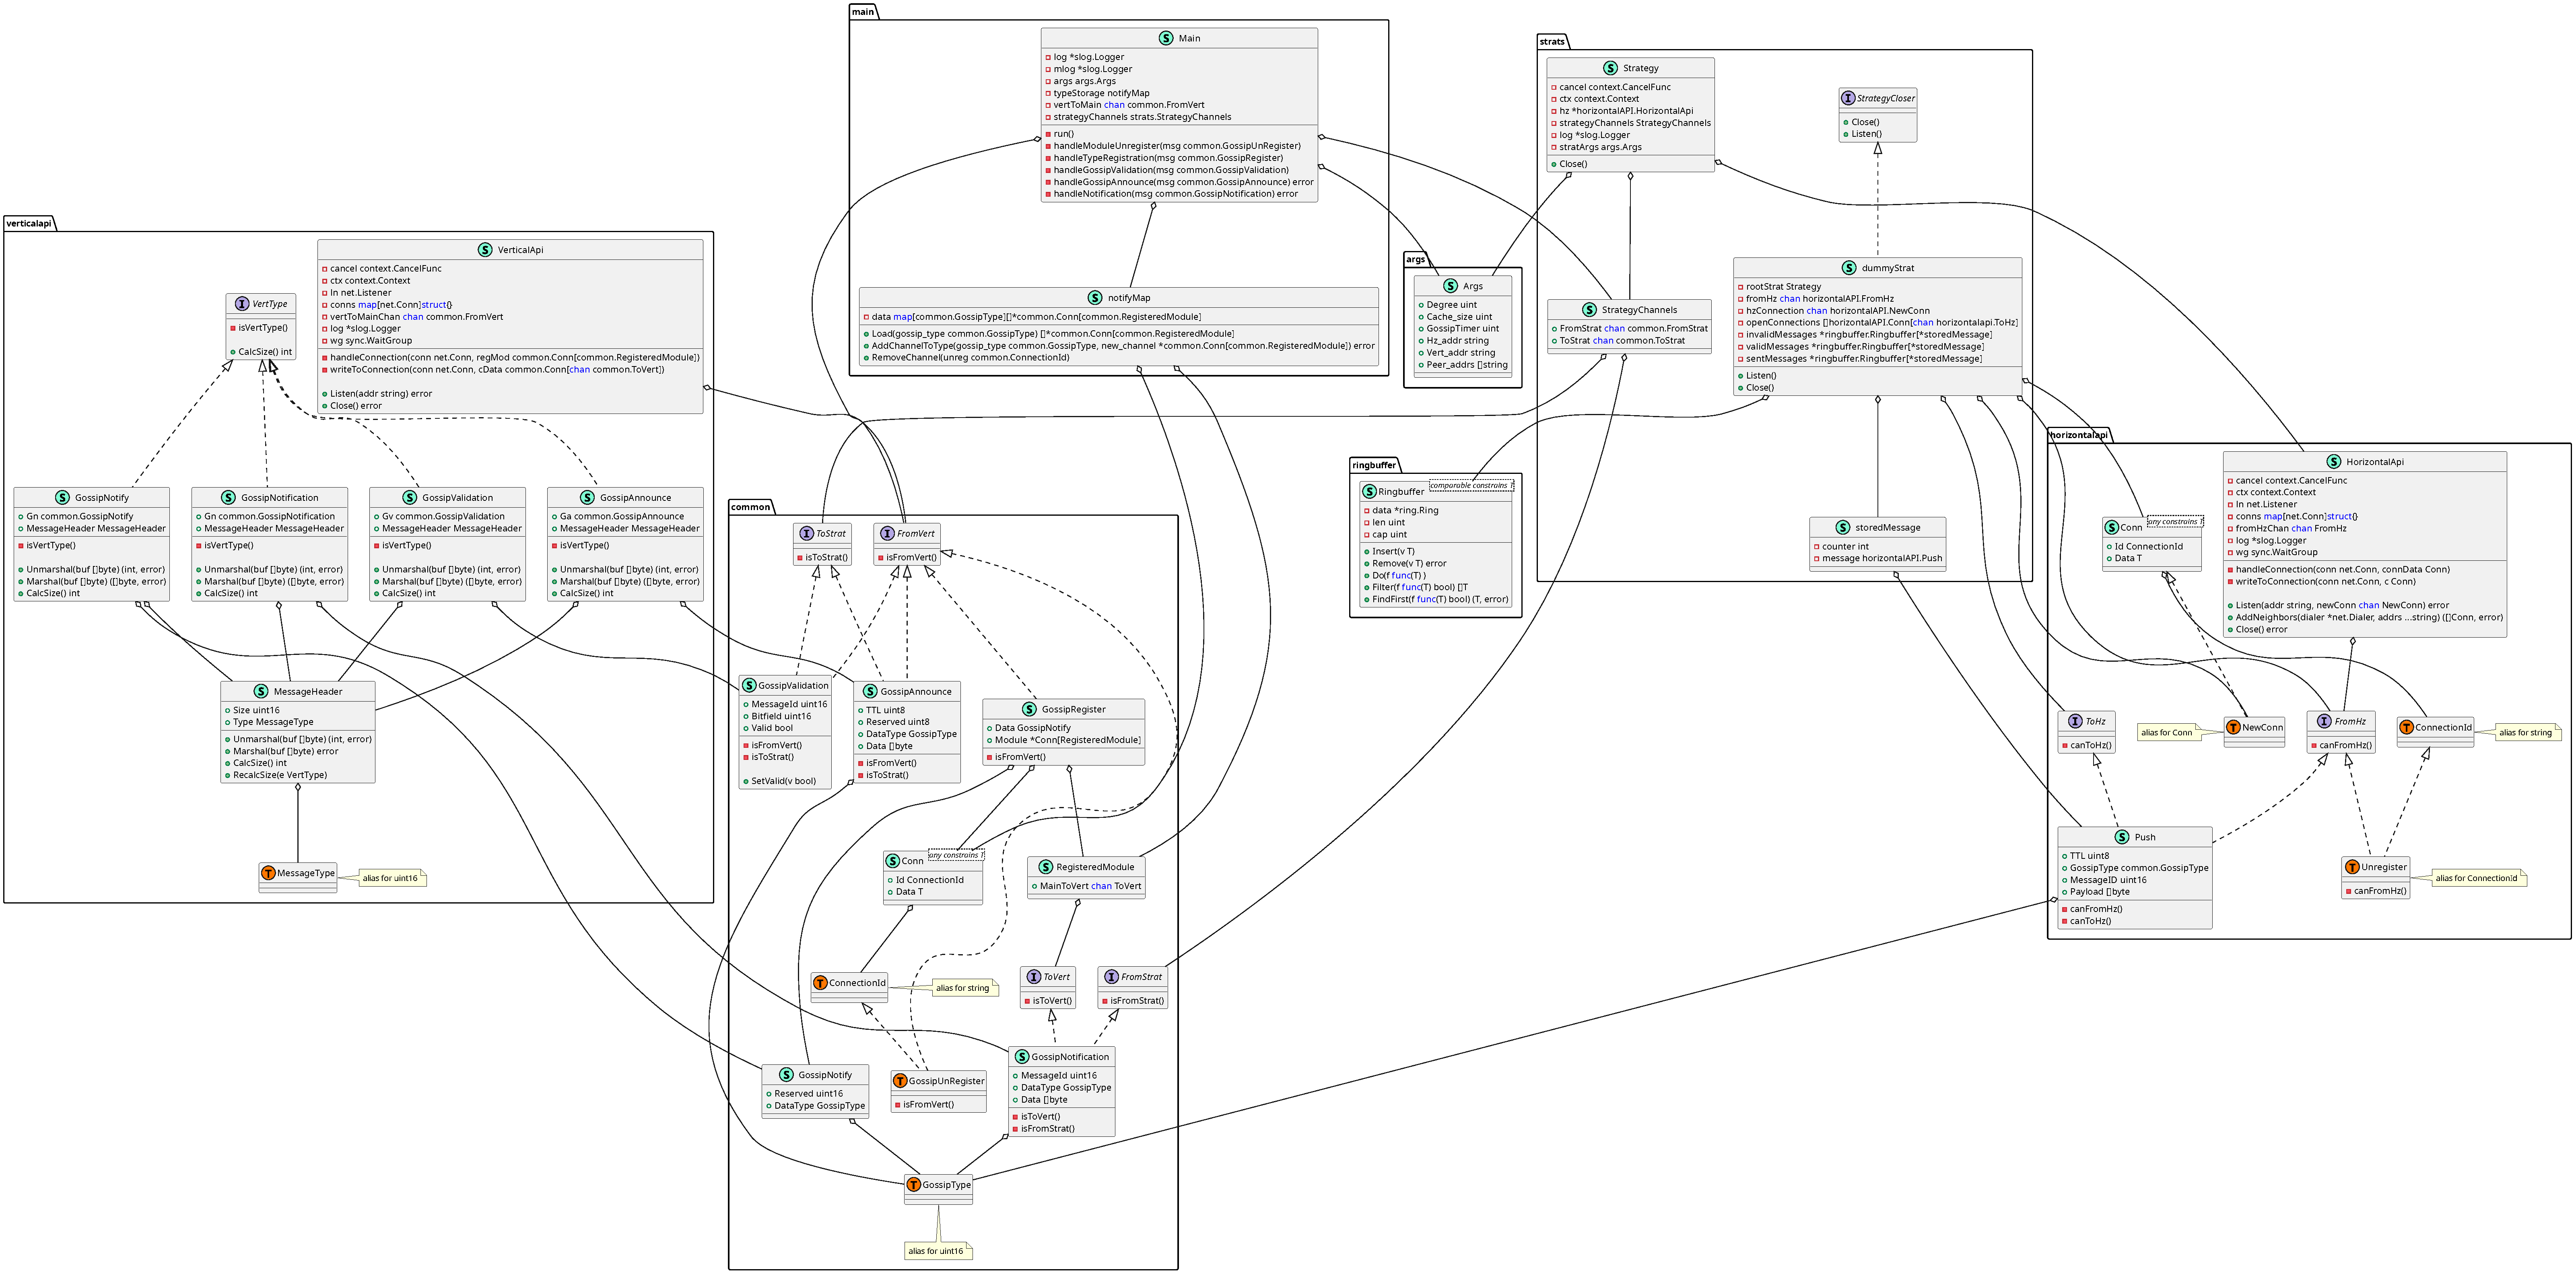
\includegraphics[width=1.2\linewidth]{figures/class}
		\caption{Class diagram for the packages included in our project, generated by PlantUML.}
		\label{fig:classDia}
	\end{figure}
\end{landscape}

\subsection{Process architecture} \label{sec:msgpassing}

To explain the current process architecture, we opted to first give a general overview of how the processes are spawned and supposed to communicate through channels. Secondly, we will display a few scenarios to show how the threads communicate with each other.

\subsubsection{Processes (threads) Creation} \label{process-creation}

\texttt{Gossip} is the entry point of the whole module. This thread spawns a listener \texttt{Vertical API} thread that keeps accepting new connection to the module from other modules following the specification of the problem statement. For each new connection, two new routines are spawned: one that receives and processes messages and one that sends messages. Communication directed to or from routines created by \texttt{Vertical API} happens respectively with channels of the \texttt{ToVert} and \texttt{FromVert} types.

Then, \texttt{Gossip} creates the \texttt{Strategy} thread, which then spawns a listener thread for the \texttt{Horizontal API}. The latter, similarly to the \texttt{Vertical API}, accepts new connection and creates for each one two threads, one for reading and one for writing. Communication between \texttt{Gossip} and \texttt{Strategy} routines happens via the \texttt{FromStrat} and \texttt{ToStrat} channels, while \texttt{Strategy} communicates with threads of \texttt{Horizontal API} via the \texttt{FromHz} and \texttt{ToHz} channels.

As already mentioned, there is actually no communication between \texttt{Horizontal API} goroutines and the \texttt{Gossip}. The channels used for communication can be seen on the arrows in \cref{fig:overview}. It is important to note that there will actually be multiple channels directed to the \textit{Vertical API} (\texttt{ToVert}), as well as multiple channels directed to the \textit{Horizontal API} (\texttt{ToHz}). This is because incoming messages from the network are aggregated on the same channel while outgoing messages are sent to specific hosts, so different channels.


\subsubsection{Scenario 1: Gossip Notify Message}

The first scenario we want to display is the reception of a Gossip Notify message. For the sake of clarity, a single Vertical API thread is used to show both the writing and reading threads.

In this case the message passing is trivial (see \cref{fig:msg-notify}). The Vertical API (\texttt{vertAPI}) receives the \textit{Gossip Notify} message (\texttt{notify}), marshals it and sends it to the main (\texttt{main}) thread where the Gossip Type is registered. It is interesting to note that what we store is the writing communication channel. As previously mentioned in \cref{process-creation}, there are multiple writing channels, one for each host. This greatly simplifies the sending procedure.

\begin{figure}
	\centering
	\begin{messagepassing}[>={Stealth[scale=1.3]}]
	\newprocesswithlength{main}{4}
	\newprocesswithlength{vertAPI}{4}
	\sendwithname{vertAPI}{1}{main}{2}{notify}
	\sendwithname{vertAPI}{1}{main}{2}{notify}
\end{messagepassing}

	\caption{Message passing when a Gossip Notify message is received}
	\label{fig:msg-notify}
\end{figure}

\subsubsection{Scenario 2: Gossip Announce Message}

In this scenario, a Gossip Announce message is sent to the Vertical API (\texttt{vertAPI}) thread. This message (\texttt{ann}) goes to the Main (\texttt{main}) module which verifies that the type is registered and if so forwards the message to the Strategy (\texttt{strat}). The strategy then sends the message to the Horizontal API (\texttt{hzAPI}) which takes care of actually sending the message to other peers. In the form of a \textit{PUSH} message. 

The delay in the Strategy, from reception to sending, is due to the implementation. Messages are sent in rounds, so they need to wait until a new sending round starts.

\begin{figure}
	\centering
	\begin{messagepassing}
	\newprocesswithlength{vertAPI}{9}
    \newprocesswithlength{main}{9}
    \newprocesswithlength{strat}{9}
	\newprocesswithlength{hzAPI}{9}
	\sendwithname{vertAPI}{1}{main}{2}{ann}
	\sendwithname{main}{2}{strat}{3}{ann}
	\sendwithname{strat}{3}{hzAPI}{4}{PUSH}	
\end{messagepassing}

	\caption{Gossip Announce message is received}
	\label{fig:msg-announce}
\end{figure}


\subsubsection{Scenario 3: Peer Relayed a Message}

In this last scenario, we depict the handling of a peer \textit{PUSH} message \cref{fig:msg-relay}. First, the message is received by the Horizontal API (\texttt{hzAPI}), then it goes to the concrete Strategy (\texttt{strat}). The strategy processes the message accordingly and asks main (\texttt{main}) to perform a Gossip Notification for such message (\texttt{notific}). If such Gossip Type is registered, Main instructs the Vertical API (\texttt{vertAPI}) to send to connected modules such message (\texttt{notific}). After that, the Vertical API receives a Gossip Validation message (\texttt{val}). On reception, this message travels the threads back to the strategy, which if the message is valid begins to spread it itself. In the figure this is the \textit{PUSH} message marked in gray. If the original message was not deemed valid, the message is not spread further.

\begin{figure}
	\centering
	\begin{messagepassing}
	\newprocesswithlength{vertAPI}{9}
    \newprocesswithlength{main}{9}
    \newprocesswithlength{strat}{9}
	\newprocesswithlength{hzAPI}{9}
	\sendwithname{hzAPI}{1}{strat}{2}{PUSH}
	\sendwithname{strat}{2}{main}{3}{notific}
	\sendwithname{main}{3}{vertAPI}{4}{notific}
	\sendwithname{vertAPI}{4}{main}{5}{val}
	\sendwithname{main}{5}{strat}{6}{val}
	\sendwithname{strat}{6}{hzAPI}{7}{PUSH}
	
\end{messagepassing}

	\caption{Peer receive \textit{PUSH} message}
	\label{fig:msg-relay}
\end{figure}


\subsection{Networking} \label{sec:structureNetworking}
For networking, we first need to differentiate between the two APIs in our module.
First, the vertical API, and second, the horizontal API.

\subsubsection{vertical API}
On the vertical API, we communicate with other modules typically running on the same peer.
At this point, these modules are implemented by someone else (\eg another team from the lecture).
Therefore, we were handed a specification that defines the format of the messages on that API.
With the hard requirement to adhere to this specification, we can't use capnproto at this point, so we need to implement the de-\,/\,parsing on our own.
If you look back at the class diagram in \cref{fig:classDia} again, this is implemented in the \texttt{verticalAPI/types} package.

\subsubsection{horizontal API}
On the other side, we have the horizontal API, which is only used for our module to communicate with the same module running on another peer.
As a result, we are completely free to come up with a custom message format on this API.
For reference on the types used, please refer to \cref{sec:msgtypes}.
In our case, we decided to use capnproto as a library that does the de-\,/\,parsing for us.
Analog to the vertical API, the code generated by capnproto is placed in the \texttt{horizontalAPI/types} package.

\subsubsection{both API-modules}
Apart from the difference in the message formats and the de-\,/\,parsing the horizontal API and the vertical API modules are quite similar.
Both modules use two threads, one for reading from and one for writing to the socket, per connection, in addition to the one thread used to establish (and dispatch) new connections.
Thereby, they both provide a layer of abstraction on top of the raw TCP sockets where other threads can send a message on the respective golang channel and (try to) receive from the golang channel in the other direction.

Especially for reading, having the golang channel is nice since we can use golang's built-in \texttt{select} statement when waiting for messages on multiple sockets.
This approach is not strictly necessary for writing.
Still, having a dedicated thread and the golang channel for communication allows us to send the message to the API module and continue execution without waiting until the message is sent on the network connection.

In general, this architecture also allows us to have multiple listening (read) and multiple writing threads connected to the API module.
We have not implemented multiple listening threads since we did not need it so far.
Also note how this use of one thread per read\,/\,write on the connection combined with the communication via golang channels implicitly synchronizes the write operations (although in golang, this is not strictly necessary to be done manually).


\section{Gossip Strategies}

The spreading of information in the network is done by the Gossip Strategy module. Since the actual way of spreading the messages could be done in many different ways (strategies), we decided to split the logic between a \textbf{Main Strategy} and a \textbf{Concrete Strategy}. There is also a class \textbf{Connection Manager} which has the task of managing the connection to the peers. 

The Main Strategy is the base component common to any Concrete Strategy. It instantiates the horizontalAPI, creates the Connection Manager object and finally the Concrete Strategy. On the other hand, a Concrete Strategy  has the job of processing incoming messages and sending its own. The whole sake of this separation is providing modularity. Our implementation offers just one strategy, the Push Strategy, but having the redundant code extracted in a common Base Class would ease in the implementation of a new strategy. That is the reason of having a Main Strategy and a Connection Manager.


\subsection{Connection Manager}

The first aspect which is in common to any Strategy is the Connection Manager. This class is responsible for abstracting the management of connections and providing a clean interface for them. This is needed due to our security measures (\cref{sec:security}), as connections have to be validated through Proofs of Work regularly. As a result, the connection state may change (e.g., a connection can become valid or invalid). These changes might occur concurrently, which could easily lead to an invalid state.

Therefore, we decided to allow changes to the internal state of connections only through a carefully exposed interface. Some of the functionalities of the Connection Manager are finding a connection for a gived ConnectionID, removing a connection or making a connection valid upon receiving a PoW.

\subsection{Gossip Messages}

\begin{figure}
	\centering
	\begin{tikzpicture}[automata]
	\node[state, initial,initial text={new mID}] (inv) {invalid};
	\node[state,accepting,right=of inv] (val) {valid};
	\node[state,right=of val] (sent) {sent};
	\node[state,below=of val] (del) {deleted};
	%
	\path (inv) edge[->] node[sloped,above] {valid=True} (val);
	\path (val) edge node[sloped,above] {sent x times} (sent);
	%
	\path (inv) edge[bend right=10] node[sloped,below] {valid=False} (del);
	\path (inv) edge[bend left=10] node[sloped,above] {cache full} (del);
	\path (val) edge node[sloped,above] {cache full} (del);
	\path (sent) edge node[sloped,above] {cache full} (del);
\end{tikzpicture}

	\caption{Finite state machine for message caching.}
	\label{fig:fsm_msgs}
\end{figure}

Ultimately, the Gossip Strategy has to receive messages, notify the verticalAPI and forward them to other peers. By specification, a received message has to be validated before it can be spread to other peers. Only then, the module can start relaying the message. After being sent to \textit{Degree} peers, there is no need to keep sending the message. 

We decided to use 3 states to describe this behavior, as described in \cref{fig:fsm_msgs}: 

\begin{itemize}
	\item \textbf{Invalid Messages}: messages that are received for the first time. The client gets notified, but they still needs to be validated by it before they can be relayed. 
	\item \textbf{Valid Messages}: messages that received a validation from the client. Now they are being spread in to other peers.
	\item \textbf{Sent Messages}: messages that were sent to \textit{Degree} peers. They are kept to avoid duplication (we could receive those messages due to a loop) and some advanced strategy could make use of them.
\end{itemize}

Those states are held in a \textbf{Ringbuffer}, a circular queue data structure which make it very easy discarding the oldest messages when the \textit{cache\_size} is exceeded. The Sent Message Queue is necessary because we can avoid loops inside the network: if an incoming message is present there, it can be automatically dropped so no loop can happen.

\subsection{Push Strategy} 
The push strategy is straight forward.
Every peer pushes new updates to a random subset of its neighbors. 

\begin{figure}
	\centering
\begin{minipage}{0.50\linewidth}
	\begin{lstlisting}[
		language=pseudo,
		morekeywords={[3]{main,hz}},
		morekeywords={[4]{msg,degree,cache\_size}},
		caption={Pseudo code of the push gossip strategy},
		label={lst:code}
	]
		on push from hz(msg):
			if msg is new (unseen) (not in any of the three caches):
				emit a notification to the main module
				mark msg as invalid for now

		on announce from main(msg):
			append msg to valid messages

		on validation from main(msg):
			if ttl == 1:
				move msg from invalid messages to sent messages
			else:
				move msg from invalid messages to valid messages

		on gossip round():
			S = random subset of the neighbors of size degree
			send all valid messages to S
			if a message was sent more than degree times:
				move msg from valid to sent messages
	\end{lstlisting}
\end{minipage}
\end{figure}

The logic is shown in the pseudocode \ref{lst:code}. Here is a more detailed explenation.

When receiving a PUSH message, two things can happen: if the message is already stored somewhere, it is immediately dropped. Otherwise, the \texttt{Vertical API} is notified and the message is marked as Invalid. The \texttt{Vertical API} has the job of forwarding the message to the client. Unless some module signals to the Gossip Strategy that the message is valid, it stays in the Invalid Queue.

If a \texttt{GOSSIP VALIDATION} message arrives, the \texttt{Gossip Strategy} will be notified. This means that a recently received message (now stored in the Invalid Queue) can be moved to the Valid Queue. If \texttt{ttl} was one, instead of being marked as Valid, the message is put in the Sent Queue. This happens because being marked as Valid means that the message will be relayed to other peers. If \texttt{ttl} is 1, the message has reached its maximum time to live, so no further relaying.

Messages received through a \texttt{GOSSIP ANNOUNCE} are automatically deemed Valid. This is because there is no client to notify and no \texttt{GOSSIP VALIDATION} to receive.

\texttt{Gossip Rounds} are triggered periodically. When the Gossip Round starts, a random subset of peers of size $\min(\text{Degree}, \text{\# neighbors})$ is chosen (via a random permutation). Then, each message in the Valid Queue is sent to each chosen peer. This way of relaying messages is just an heuristic: on average the message should reach all peers within the \texttt{ttl} but it is not guaranteed. If the amount of connection a peer has is bigger than \textit{Degree}, some neighbors will not receive the PUSH message and there is no guarantee they will receive it later. But the specification says that a peer should exchange information with \textit{Degree} peers, so it is also responsibility of the users to choose an appropriate \textit{Degree} number.


\section{Security Measures} \label{sec:security}

From a security perspective, the Gossip module is mainly susceptible to \textit{Sybil Attacks} and consequently \textit{Eclipse Attacks}. This is because, when running, a peer is accepting any new connection and there is no central authority which can help with verifying the identity of other entities. To provide Identity Validation we opted for a computation based Proof of Work. This way we limit the amount of Identities which can be under the control of an attacker to the computational resources that such attacker has. 

\subsection{Identity Validation}

The act of validating identity in our system involves solving a Proof of Work (PoW) challenge. Specifically, this means finding a nonce (a random or pseudo-random value) that, when appended to a given challenge, results in a hash output with a specified number ($n$) of leading zeros. This process is similar to the one of the registration challenge.

The purpose of this PoW mechanism is to ensure that the client has invested computational effort in proving its legitimacy. Once the correct nonce is identified and appended to the challenge, any peer can verify such PoW efficiently: if the hash function generates an output that starts with the required number of leading zeros, the Proof of Work is considered valid.

This mechanism provides security by making it computationally expensive to forge identities or spam the system with invalid connections (\textit{Sybil Attacks}). 

The difficulty of the challenge, controlled by the number of leading zeros $n$ required in the hash, can be adjusted based on the desired level of security. Higher numbers of leading zeros require more computational work, making the system more secure but also more resource-intensive. But the difficulty can also be raised by putting a (small) time constrain for the computation of such PoW.

In our project, $n$ is set to 8 bits, meaning the hash must start with 8 leading zeros. However, the optimal security parameters can only be determined by running the nodes in a real test environment. Various combinations of timeout lengths and the number of leading zeros may be suitable, depending on the specific circumstances.

\subsection{PoW Protocol Design}

The Proof of Work happens through the exchange of Horizontal messages. To explain how we designed the Identity Validation protocol, let's go through an example. Peer $R$ (receiver) is up, and peer $I$ (initiator) is instructed to connect to peer $R$:

\begin{enumerate}
	\item $I \to R$ send a request. The message only purpose is to instruct $A$ of creating and providing a challenge
	\item $R \to I$ send a challenge. 
	\item $I \to R$ send the Proof of Work. If valid, the Identity is validated
\end{enumerate}

\begin{figure}
	\centering
	\setlength\mySkip{2ex}
\begin{tikzpicture}[
	auto,>=stealth',
	status/.style={TUMBlue,},
	statusR/.style={status,below right},
	statusI/.style={status,below left},
	thick,
	]

	\node (i) {Initiator};
	\node[right=3cm of i] (r) {Responder};

	\node[fit=(i) (r),inner sep=0pt] (tmp) {};
	\coordinate[yshift=-3ex] (tmp) at (tmp.south);

	\draw[<->] (tmp -| i) -- node[above,scale=1,midway]{Connection Establishment} (tmp -| r);
	\node[statusR] (sR) at (tmp -| r) {in progress};
	\node[statusI] (sI) at (tmp -| i) {to be proved};

	\node[fit=(sR.south) (sI.south),inner sep=0pt] (tmp) {};
	\coordinate[yshift=-\mySkip] (tmp) at (tmp.south);

	\draw[->] (tmp -| i) -- node[above,scale=1,midway]{ConnReq} (tmp -| r);
	\node[statusR] (sR) at (tmp -| r) {in progress};
	\node[statusI] (sI) at (tmp -| i) {to be proved};

	\node[fit=(sR.south) (sI.south),inner sep=0pt] (tmp) {};
	\coordinate[yshift=-\mySkip] (tmp) at (tmp.south);

	\draw[<-] (tmp -| i) -- node[above,scale=1,midway]{ConnChall} (tmp -| r);
	\node[statusR] (sR) at (tmp -| r) {in progress};
	\node[statusI] (sI) at (tmp -| i) {to be proved};

	\node[fit=(sR.south) (sI.south),inner sep=0pt] (tmp) {};
	\coordinate[yshift=-\mySkip] (tmp) at (tmp.south);

	\draw[->] (tmp -| i) -- node[above,scale=1,midway]{ConnPoW} (tmp -| r);
	\node[statusR] (sR) at (tmp -| r) {open connection};
	\node[statusI] (sI) at (tmp -| i) {open connection};

	\node[fit=(sR.south) (sI.south),inner sep=0pt] (tmp) {};
	\coordinate[yshift=-\mySkip] (tmp) at (tmp.south);

	\draw (i.south) -- (i.south |- tmp);
	\draw (r.south) -- (r.south |- tmp);

\end{tikzpicture}


	\caption{
		Sequence Diagram of the PoW protocol on connection establishment.
		The \textcolor{TUMBlue}{blue labels} refer to the state the connection currently is in from the point of view of the respective peer.
	}
	\label{fig:seqPow}
\end{figure}
\subsubsection{Connection Types}

To better model the PoW, we decided upon 3 possible connection state:

\begin{enumerate}
	\item \texttt{To Be Proved Connections}: peers to which a PoW needs to be sent. Those are supplied at startup.
	\item \texttt{In Progress Connections}: peers which need to send us a PoW. Those are connection initiated by other peers.
	\item \texttt{Open Connections}: peers that were validated (or we validated us against).
\end{enumerate}

For each To Be Proved connection, a peer will send a \texttt{ConnReq} message. Upon reception of \texttt{ConnChall} messages (the challenges), it will compute the PoW and send it as a \texttt{ConnPow} message. After that the connection will become a Open one (valid).

From the other perspective, if \texttt{ConnReq} are coming from In Progress Connections, a peer will reply with challenges. When receiving a \texttt{ConnPoW} message, if the PoW is valid, the peer il make such connection Open (valid). 

These states become handy when receiving and handling PoW messages, as we must verify that a message is coming from a connection in a specific state. For example, we only accept Challenges if the connection is a To Be Proved ones. Or we automatically drop PUSH messages if the connection is not a valid one (not present in the Open Connections).

\subsubsection{Solving the Proof of Work}
For the proof-of-work we are using a scheme similar to the one used in the registration challenge.
So the peer is required to return a nonce which leeds the hash digest of a structure (containing the nonce) to fulfill a certain predicate.
Usually the prodicate is that the digest needs to start with a null byte.
The generic solver we wrote for this can be used to solve the proof-of-work for any structure and also with an arbitrary predicate.
The only caveat is, the nonce needs to be located at the end of the structure.
The reason behind this caveat is that the generic solver makes use of the \href{https://en.wikipedia.org/wiki/Merkle\%E2\%80\%93Damg\%C3\%A5rd\_construction}{Merkle-Damg\aa rd Construction} quite similar to the \href{https://en.wikipedia.org/wiki/Length\_extension\_attack}{length extension attack} to speed up the calculation by reusing the internal state of the hash function.
Additionally, we made the solver to work with multiple workers running in parallel.

In our case, the hash digest of the proof-of-work is calculated over the complete cookie (see \cref{fig:cookie}) followed by the nonce which solves the proof-of-work.

\subsubsection{Cookies}

\begin{table}
	\centering
	\begin{tabularx}{.85\linewidth}{llX}
	\toprule
	ChaCha20 Nonce & IP and PORT & timestamp 
	\\
	\bottomrule
\end{tabularx}
	\caption{Cookies content}
	\label{fig:cookie}
\end{table}

When a peer is validating an incoming connection, some information should be maintained in memory. This can be leveraged by an attacker: he could open many connections, and leave them half done (not providing the PoW) thus increasing the memory load on the peer much like a TCP SYN Flood attack. To avoid this kind of attack, we opted for the use of cookies which avoids keeping state in memory at the responder.

The cookie content is shown in \cref{fig:cookie}. It is composed of a clear text part and an encrypted one. The encrypted part contains a timestamp, the Nonce used by the encryption algorithm, and the destination address (Ip and Port number) of the peer which needs to ba validated. The clear text part just contains the Nonce for the encryption algorithm.

ChaCha20-Poly1305 \footnote{\url{https://en.wikipedia.org/wiki/ChaCha20-Poly1305}} was chosen as the encryption mechanism providing AEAD. Even though we don't use the Associated Data this still provides us with authenticated encryption. The used key is randomly generated at startup by each peer.

Upon reception of the PoW, which contains the cookie and a Nonce for the pow computation \label{tab:pow}, the Cookie is decrypted. If the decryption fails, the connection is immediately dropped. Otherwise, the content of the cookie is inspected for additional checks. For example, the timestamp should not be larger than a certain timeout value, as we don't allow a peer to take arbitrary time to compute the PoW.

\subsection{Periodical Proofs of Work} \label{sec:periodic}

The PoW requires an attacker to put in computational effort when opening a connection. But if this is done only once, the attacker can use the resource sequentially, adding Sybils under its control over time. To mitigate this, we implemented Periodic Proofs of Work. A node periodically asks the neighboring peers for a PoW and at the same time, the node will be prompted by each of its neighbors for PoWs. 

We have previously thought about aggregating the received Challenges into a single PoW so that a node does not waste too many resources in multiple PoWs. Otherwise, we would penalize nodes that have many connections. At the same time, by aggregating, an attacker could open as many connections as he wants paying the same computational cost. In the end, we opted for providing PoW for each connection. This has a higher load on the peers but provides the best security against Sybils.

The Periodic PoW is specular to the previously illustrated ones. There are two timers, one for requesting challenges to all Open Connections (valid ones) and one for closing connections which did not provide the Periodic PoW. The former must be shorter than the latter (at least half) as there is no synchronization between peers.  

\subsubsection{DoS Protection}

One of the caveats of the Proof of Work is that there must be some mechanism which controls when a PoW is calculated. If none is in place, an attacker can ask for an indefinite amount of PoWs, effectively performing a DoS attack on the target peer. 

During connection establishment, this is done by accepting challenges only from peers we want to connect to. For the Periodic Proof of Work, it is not possible anymore since all messages originate from the same class of connections (valid ones).

To prevent DoS attacks, we keep track of sent requests: a Challenge is accepted only if a request was previously sent. In this case, it is not needed to use cookies, as the Open (valid) connections have been proved, and the risk of a Flood type of attack is way smaller.

\section{Specification of the peer-to-peer protocol} \label{sec:msgtypes}

This module works with two protocols, one on the vertical API and one on the horizontal API.
The one for the vertical API was already predetermined.
Its specification can be found in the \emph{specification.pdf} document (see moodle\footnote{\url{https://www.moodle.tum.de/mod/resource/view.php?id=3090766}}).
For the other one, we had the freedom to develop something independently.
To avoid writing the de-\,/\,parsing ourselves, we chose to use capnproto.
Capnproto is a data serialization format that comes with libraries in multiple different languages and a respective code generator for those languages.
With capnproto, you only specify what data (\enquote{name} and type) should be in the message.
The concrete message format is then the concern of capnproto.

With this in mind, it makes no real sense to include the concrete format of the messages but only the names of the fields and their type.
% TODO(pull)
As of now, we have seven message types on the horizontal API.
The most important one is the \emph{Push} message type, which is used to spread information in the network.
Its fields and types can be seen in \cref{tab:push}.

The six remaining message types can be split into two groups, one with the \emph{Conn} prefix and one with the \emph{Pow} prefix.
Both groups are of size three.
Regarding the payload, both sets of message types are equal.
We use different message types nonetheless since we use them in a slightly different context and want to be able to differentiate what message exactly was sent.
Both sets of message types consist of
a \emph{Req} message type (see \cref{tab:req}),
a \emph{Chall} message type (see \cref{tab:chall}) and
a \emph{Pow} message type (see \cref{tab:pow}).
All of them are used for our security mechanism.
For more information on this mechanism, please refer to \cref{sec:security}.

The actual message sent on the horizontal API is not a raw instance of the message described above but a more generic message type, which is a simple union of all message types that can be sent on the horizontal API.
This approach makes it possible to add more message types as we go by simply adding more types to this union.
The nice thing at this point is that capnproto handles the complete checking of which message type was sent (resolving the union, so to speak).
This way, we do not need to come up with, \eg a messageType field on our own and allocate identifiers for the individual types.

\begin{table}
	\centering
	\begin{tabularx}{.85\linewidth}{llX}
	\toprule
	Field & Type & Description
	\\
	\midrule
	ttl & Uint8 & Time to live: specifies nodes until which distance to the transmitting node should be reached ($\text{TTL} = 0 \text{ means } \infty$)
	\\
	gossipType & Uint16 & Type of the payload (set by the module talking on the verticalAPI)
	\\
	messageID & Uint16 & Identifier of this message (randomely chosen by the strategy)
	\\
	payload & Data & Bytes of data that is spread in the network
	\\
	\bottomrule
\end{tabularx}

	\caption{
		Contents of a \texttt{Push} message.
		Used to spread information.
	}
	\label{tab:push}
\end{table}

\begin{table}
	\centering
	\begin{tabularx}{.85\linewidth}{llX}
	\toprule
	Field & Type & Description
	\\
	\midrule
	\multicolumn{3}{l}{No payload needed as this only serves to request a challenge for the proof-of-work.}
	\\
	\bottomrule
\end{tabularx}

	\caption{
		Contents of a \texttt{\{Conn,Pow\}Req}* message.
		Used for the security mechanism.
	}
	\label{tab:req}
\end{table}

\begin{table}
	\centering
	\begin{tabularx}{.85\linewidth}{llX}
	\toprule
	Field & Type & Description
	\\
	\midrule
	cookie & Data & a cookie for this request, serves also as challenge for the proof-of-work
	\\
	\bottomrule
\end{tabularx}

	\caption{
		Contents of a \texttt{\{Conn,Pow\}Chall} message.
		Used for the security mechanism.
	}
	\label{tab:chall}
\end{table}

\begin{table}
	\centering
	\begin{tabularx}{.85\linewidth}{llX}
	\toprule
	Field & Type & Description
	\\
	\midrule
	nonce & uint64 & nonce which solves the challenge of the proof-of-work
	\\
	cookie & Data & cookie of the original request, serves as challenge in the proof-of-work
	\\
	\bottomrule
\end{tabularx}

	\caption{
		Contents of a \texttt{\{Conn,Pow\}PoW}* message.
		Used for the security mechanism.
	}
	\label{tab:pow}
\end{table}

\section{Testing} \label{sec:testing}
Testing can be split into multiple categories.
In this project, we make use of unit testing and end-to-end testing.
Both kinds of tests are written in files suffixed with \texttt{\_test.go}.
Therefore, if you use \lstinline{go test} to run the tests, both kinds of tests are executed.

You will find the files containing the unit tests placed side-by-side the files containing the code they test.
Unit testing is straightforward and will not be covered in more detail in this documentation.

For the end-to-end testing, we came up with a more complex setup that relies on a \texttt{Tester} class (see \texttt{internal/testutils/}) for the most part.
You will find the specification of the test cases in \texttt{gossip/main/main\_test.go}.
But now let us focus on the \texttt{Tester} class used in the process.

The basic idea for end-to-end testing is to bring up multiple instances of our application, one for each node in a network.
The topology of the network is defined beforehand in a JSON file.
Afterward, we can instruct one instance to spread information in the network, and we can observe how the nodes in the network handle this.

In order to do so, we create multiple goroutines, one for each node, and launch our application with the respective configuration in each of these goroutines.
To observe the process, we set up each instance to output its logs in JSON format and output log statements with a predefined log level (only used for this kind of testing).
We can then parse the redirected JSON log output in the testing routine and collect it for later use.
Additionally, for each node, we open a TCP connection for the vertical API to control the node, just like in a real-world scenario.

All this functionality is implemented in the \texttt{Tester} class.
\texttt{NewTesterFromJSON} parses the JSON file defining the topology,
\texttt{Startup} starts the application multiple times and opens the vertical API connections, and
\texttt{Teardown} closes all the connections and terminates all instances.
Having all these functionalities collected in one class has the advantage that we can use it for multiple different test cases.

For ease of use, we added more functions to the \texttt{Tester} class.
One example is registering a certain \emph{gossipType} on all nodes so that all nodes participate in spreading the information.
Another example is waiting until no more messages are sent (for a particular duration) on the horizontal connections (except for PoW messages).
The latter is particularly useful when waiting until the information was spread before calling \texttt{Teardown}.

Writing all this in golang has the advantage of simply reusing the struct definitions of our project.
This is particularly useful when sending messages on the vertical API.
Also, this makes integrating the tests in the golang way of running tests easier.

The goal was to provide a layer of abstraction on top of the whole management of the nodes so that the actual test case is just a simple playbook of what should happen.
Therefore, if you look at the end-to-end tests, they read very script-like.

The \texttt{Tester} was also designed to be used for some benchmarks.
In this case, the approach of using a predefined log level comes in handy as it allows the placement of various hooks in the codebase, which can later be used during benchmarking.
We already started looking at, \eg which node receives the information when and how many packets are sent at which point in time.
For this reason, you will already find some code regarding analyzing of the gathered data in the \texttt{Tester} class.
However, as randomness is involved in the gossip strategy, coming up with good metrics is quite challenging.
This is why, in the end, we did not perform extended benchmarking, providing us with results we can present at this point.
\Cref{fig:reachedWhen} and \cref{fig:packetsOverTime} show two visualizations of the data we currently collect from one test run.

\begin{figure}
	\centering
	\begin{tikzpicture}
	\begin{axis}[
		font            = {\small},
		line width      = {0.2pt},
		width           = {.5\linewidth},
		legend style    = {at={(xticklabel cs:0.5)},yshift=-4ex,anchor=north},
		% legend columns  = -1,
		grid            = major,
		grid style      = {gray!30},
		axis lines      = middle,
		axis line style = {->,> = {Stealth[scale=1.75]}},
		x label style   = {at={(xticklabel cs:0.5)},anchor=north},
		y label style   = {at={(yticklabel cs:1)},yshift=3ex,anchor=south west},
		xmin = 0,
		xlabel = {Time [s]},
		ylabel = {cnt Packets},
		ybar,
		enlargelimits=true,
		]
		\addplot+[] table[x=TimeUnixSec,y=Cnt,col sep=comma] {figures/packets_sent.csv};
		\addlegendentry{Packets sent over time}
	\end{axis}
\end{tikzpicture}

	\caption{
		Example plot of benchmarking data.
		Shows how many packets are sent over time in the complete network.
		In this test, only one information message with TTL~3 was inserted to the network leading to multiple push messages and proof-of-work messages.
	}
	\label{fig:packetsOverTime}
\end{figure}

\begin{figure}
	\centering
	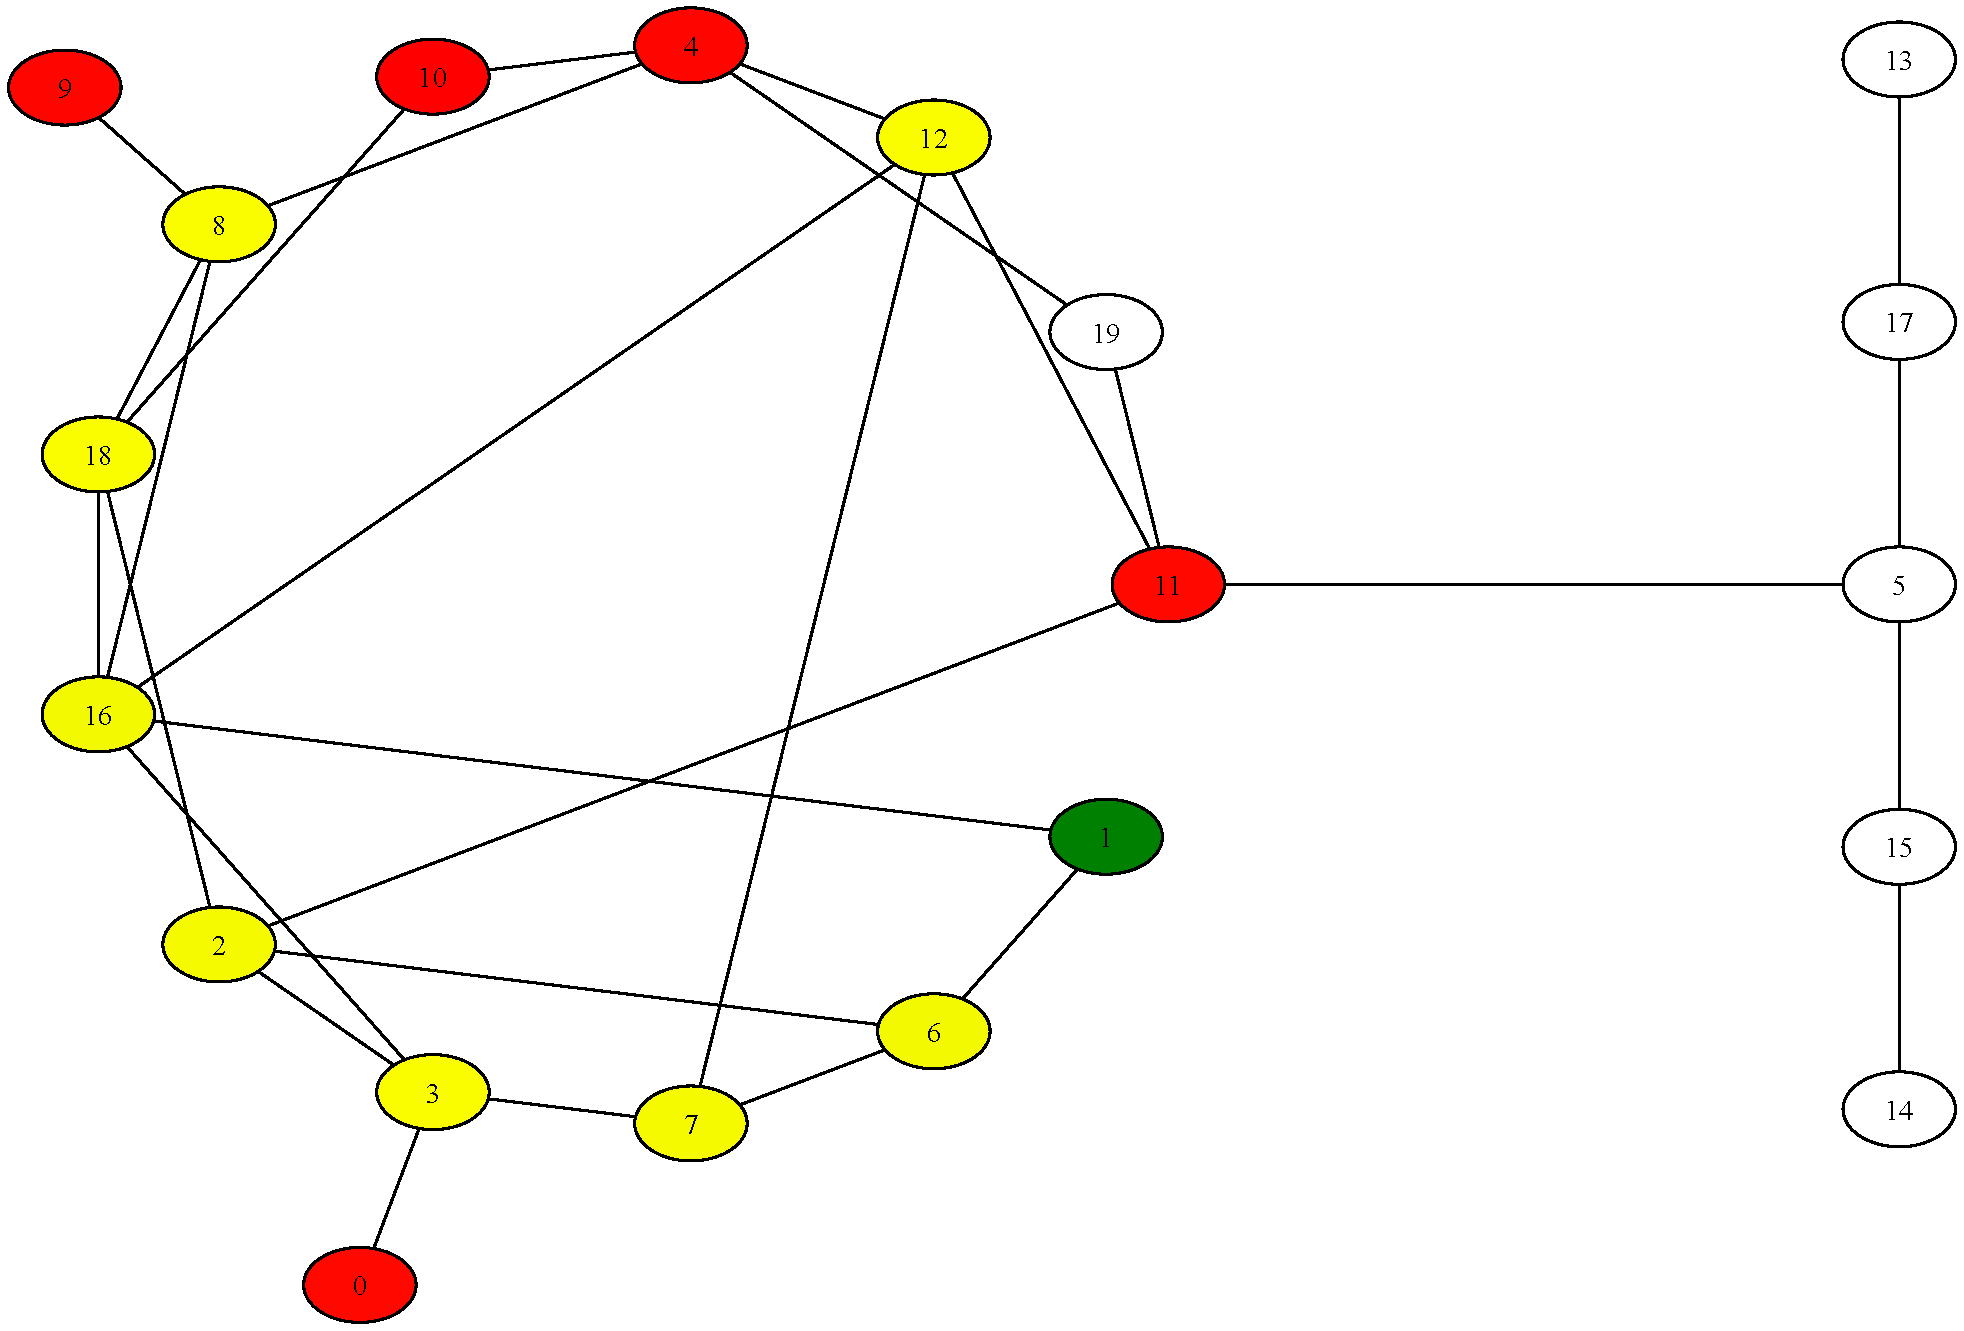
\includegraphics[width=1\linewidth]{figures/reached_circo.pdf}
	\caption{
		Example figure with benchmarking data.
		Shows color coded when which peer received the information.
		In this test, one announcement was sent to node~1 with TTL~3.
	}
	\label{fig:reachedWhen}
\end{figure}

\section{Future Work} \label{sec:future}

With this project, we built a solid architecture with significant attention to modularity. Handling new Horizontal Messages or creating new Gossip Strategies is not only possible but foreseen by the architecture. For example, for writing a new Gossip Strategy, the Main Strategy can be leveraged, and the user can focus only on the logic of such Strategy. In this section, we will present features we would have implemented if we had given more time to focus on the project.

\subsection{Pull Strategy}

A PUSH only strategy has flaws. It can happen that information does not reach all peers. We planned on adding a PULL protocol to increase the probability that all peers would eventually receive all messages. By adding, we mean integrating the already in place PUSH Strategy with PULL messages. The general idea is made of 3 steps for a given peer:

\begin{enumerate}
    \item Choose a number of neighbors
    \item Send a PULL message (request) to those neighbors
    \item Receive and merge the new messages, sent as a PULL response
\end{enumerate}

For the first step, how to choose a neighbor would be at random. Another possibility would be to select a neighbor that has not sent many PUSH messages, meaning that it might have stored messages that did not reach this peer.

For the second and the third, we had a few ideas in mind. A simple method would be for the responder (the neighbor) to send the $n$ most recent messages. A more complex strategy would have the initiator peer sending a list of message IDs it has in memory; the responder would compare the list with its own, looking for new messages not present, and then send those new messages to the Initiator.

Ultimately, these ideas could have all been implemented and later evaluated using benchmarking (see \cref{fut:benchmarking}).

\subsection{PUSH Proof of Work}

A possible security flaw we have not addressed is the one about spamming. With the Periodic Proof of Work (\cref{sec:periodic}), we make sure that every identity is validated by possessing a certain amount of computing power. However, an attacker who owns one valid peer could still send an arbitrary number of PUSH messages.

We have thought about limiting the global amount of PUSH messages by implementing a Proof of Work for each PUSH message. Since PUSH messages would come without a request (that would overly complicate the protocol), we thought about crafting unique payloads for PUSH messages on which to compute the PoW. Such payload would consist of:

\begin{itemize}
    \item The message, which is sent anyway
    \item The destination IP and Port, so an attacker has to compute the PoW for each connection
\end{itemize}

This way of computing the PoW does not prove the freshness of the message: an attacker could pre-compute 100 different messages and then send them all at once. But at least it could not spam them over all neighbors.

In the end, we did not explore this security measure as there is no real way of assessing whether messages are spam or legitimate. Moreover, it would greatly increase the load on peers as each PUSH message should have a PoW. It would be a tradeoff between performance and security.

\subsection{Benchmarking} \label{fut:benchmarking}
Usually, benchmarking is used to evaluate the performance of an application.
Also, benchmarking can be used to compare the performance of using different parameters.
In this project, we already included some means to ease the writing of test scenarios and to retrieve \eg how many packets are sent or which nodes obtain knowledge of a certain information (see \cref{sec:testing}).
For benchmarking, a large random topology shall probably be used, which cannot be configured by hand.
In order to automatically generate such a configuration, we wrote a small python script using the networkx\footnote{\url{https://networkx.org/}} library.
Despite all the progress made, proper benchmarking is still to be done.
The biggest challenge here is deriving stable metrics with all the randomness involved.
With stable we mean that the metric does not change significantly when rerunning the benchmark.

\section{Workload distribution}
As already outlined, we split our module in various different packages.
This enabled us to distribute the packages and work independently of each other (apart from defining the communication\,/\,interface of course).

Fabio focused on the developing the Strategy package, which was initially written in peer programming, especially when defining the whole interface. He implemented the Cookie and Gossip Connection. He also wrote the tests for the vertical API and developed the most part of the PoW security mechanism.

Lukas worked on the horizontal API and the vertical API (from which the common package later was derived).
Note that at least writing the de-\,/\,parsing of the vertical API was pretty straight forward because it is fairly similar to what we needed to do for the registration client.
He also wrote the module which is used to solve the PoW challenge (in parallel) and developed the capabilities for easy end-to-end testing (and the stubs for benchmarking).

While Fabio started working on the main package, Lukas later did some refactoring and finalized the package.

\section{Effort spent for the project}
Both of us did not strictly measure the time spent on the project. We report here a rough estimation on weekly hours spent working on the project, since the creation and submission of the initial report.

\todo{I (Fabio) counted 70 hours except today}

\begin{itemize}
	\item Fabio: 7-8 hours a week
	\item Lukas: 7-8 hours a week
\end{itemize}

We would like to point out that this estimation is an average.
There were weeks where one member did slightly less and weeks when he did more.
Moreover, it is not the case that those hours were spread equally across the week, but rather done in 3-4 hours long session (in a few occasion a bit more).
Also, sometimes these were pair-programming sessions or sessions for planning where the architecture was planned (and almost no code was written).
Especially after the lecture period ended Fabio was able to put more effort into the project while Lukas worked more on the project arround the exam phase.

\todos

\end{document}
